\chapter{Results and Analysis}
\label{ch:resultsAndAnalysis}

\section{Data collection and generation}%
\label{sec:data_collection_and_generation}

We now discuss how the real-world data is retrieved and preprocessed as well as
presenting some techniques for generatic synthetic data.

\subsection{Collection and preprocessing}%
\label{sub:collection_and_preprocessing}

Datasets are built mainly upon $2$ social medias: Twitter and Reddit; the data
collection process, consequently, slightly differ between them.

\paragraph{Twitter}%
\label{par:twitter-data}

Twitter's \emph{Interaction Graphs} are mainly built starting from the tweets
of some important social accounts associated to well-known news source, like The
New York Times or Fox News, that tipically post links to their articles:
these profiles are taken as the source of the contents $\mathcal{C} $ of the graph.

Each time another user tweets the same url (\autoref{fig:twitter-thread}) then
it will correspond to another thread related to the same content, and all the
replies it receives will be part of this new thread.

Twitter data is retrieved with the help of Tweepy \cite{tweepy}, a Python
library for accessing the Twitter API, which has been patched for using some
features available only in the beta of the new Twitter API (v2).

\paragraph{Reddit}%
\label{par:reddit}

Differently from Twitter, Reddit focuses on subreddits, which are pages
collecting posts from different users about a specific topic (e.g. r/politics,
r/economics, $\dots$). This means that
in the datasets built from this social media the contents $\mathcal{C} $ is the
set of posts of these pages, which, differently from Twitter, most likely
come from different sources.

This posts are in turn crossposted, i.e. reposted on other subreddits. Each of
these \emph{crosspost} will eventually correspond to another thread.

The PRAW library is used for retrieving the data \cite{praw}.

\paragraph{Edge weights assignment}%
\label{par:assigning_edge_weights}

Once the threads interactions are retrieved they are passed to a state of the
art sentiment analyzer which labels them. More specifically the model used is
RoBERTa which has been adapted and retrained for dealing with Twitter
data \cite{Barbieri2020}. The model is made available by the Transformers
python library \cite{wolf-etal-2020-transformers}.

\bigskip

Finally, complying with the current privacy legislation, all the data related
to the user is pseudo-anonymized (accounts identifier are replaced by random
ones) while no data is publicly available.

\subsection{Synthetic data}%
\label{sub:synthetic_data}

Here we propose $2$ possible methods for generating data, the Signed SBM and
the Information spread Model.

\subsubsection{Signed SBM}%
\label{ssub:signed_sbm}

This model is very similar to the Stochastic Block Model (SBM), a model
commonly used for generating random graphs having some community structures
\cite{Newman2018}.

The Signed SBM is based on the following parameters
\begin{itemize}
	\item $b_{i} $, the group assignment of each vertex $i$
	\item $\omega ^{+} _{rs} $ and $\omega ^{-} _{rs} $, the probabilities
	      of positive and negative edges, respectively, between users in
	      group $r$ and $s$. Vertices have also a probability of not having an
	      edge, which is equal to $1 - \omega ^{-} _{rs} - \omega ^{+} _{rs} $.
	      For this reason it is clearly needed that $\omega ^{+} _{rs} + \omega ^{-} _{rs} \leq 1$.
	\item $\theta \leq 1$, controlling the reduction of probability of interacting
	      between \emph{inactive} communities
\end{itemize}

Therefore, generating a thread layer\footnote{in this model we will generate contents univocally associated to threads} for the \emph{Interaction Graph} involves the following process
\begin{enumerate}
	\item Sample $n'$ among the $n$ communities. These are the
	      \emph{active} communities in the discussion of the thread
	\item For each node pairing $i, j$ consider their corresponding groups $r$ and
	      $s$ and draw from one of the following categorical distribution to decide to add
	      a positive, negative or no edge.
	      \begin{itemize}
		      \item If both communities $r$ and $s$ are \emph{active}
		            \begin{equation*}
			            (\omega _{rs} ^{+}, \omega _{rs} ^{-}, 1 - \omega _{rs} ^{+} - \omega _{rs} ^{-})
		            \end{equation*}
		      \item otherwise
		            \begin{equation*}
			            (\theta \omega _{rs} ^{+}, \theta \omega _{rs} ^{-}, 1 - \theta (\omega _{rs} ^{+} + \omega _{rs} ^{-}))
		            \end{equation*}

	      \end{itemize}

\end{enumerate}

\subsubsection{Information spread model}%
\label{ssub:information_spread_model}

Here we describe the Information spread model, which aims at simulating the
process of informations flowing between different users of a social media.

Like in the Signed SBM, each node has a group assignment and there are probabilities of
positive and negative edges $\omega _{rs}^{+}  $ and $\omega _{rs}^{+}  $,
respectively, with $\omega ^{-} _{rs} + \omega ^{+} _{rs}
	\leq 1$. Additionally, we have the following new parameters

\begin{itemize}
	\item ${\phi_{rs} }$, the parameters of a standard SBM
	\item $\beta _a$, the probability that a node is initially activated
	\item $\beta _n$, the probability the an inactive node is activated
	      from a friend
\end{itemize}

\bigskip
Generate the \emph{follow} graph $G_{f}$ from a SBM with parameters $\{ \phi
	_{rs}  \}$; we will refer to neighbours in this graph as \emph{friends}.
The generation of a thread for the \emph{Interaction Graph} goes as follows

\begin{enumerate}
	\item Activate vertices with probability $\beta_{a}  $
	\item Any of these active nodes activates its inactive friends with
	      probability $\beta_n$
	      % \item Let $a_{i} $ be the number of \emph{active} neighbours of node
	      %     $i$ in $G$ and $m_{i} $ the number of neighbours of node $i$ in
	      %     $G$. Any node inactive from the previous step is activated with
	      %     probability $ \frac{a_i}{m_i} \beta _{n} $
	\item Similarly to before, if $2$ nodes are both active nodes they will interact according to the categorical distribution
	      \begin{equation*}
		      (\omega _{rs}
		      ^{+}, \omega _{rs} ^{-}, 1 - \omega _{rs} ^{+} - \omega _{rs} ^{-})
	      \end{equation*}

	      otherwise according to
	      \begin{equation*}
		      (\theta \omega _{rs} ^{+}, \theta \omega _{rs} ^{-}, 1
		      - \theta (\omega _{rs} ^{+} + \omega _{rs} ^{-}))
	      \end{equation*}
\end{enumerate}

\section{Major results}

The following presented results have been obtained from a Python
implementation of the methods decribed in the previous chapters. The library used
for handling and manipulating graphs is graph-tool, which has been chosen
because of its efficiency \cite{peixoto_graph-tool_2014}.

\subsection{Initial Real-world data analysis}%
\label{sub:validity_problem_definition}

We did a initial analysis of the data to verify the validity of the problem. We
initially analyzed the $\eta(C)$, more specifically its distribution, and
compared it with the distribution of the $\eta(T)$. We report these results for
$2$ datasets, one built over @nytimes and another over @foxnews Twitter
accounts \footnotemark (\autoref{fig:eta-content-thread}).

\footnotetext{As explained above (\autoref{par:twitter-data}), we are referring
	to the accounts that are used to retrieve the contents of the graph}

% todo correct CNN image and discussion of these results

\begin{figure}
	\begin{center}
		\begin{subfigure}[b]{0.4\textwidth}
			\centering
			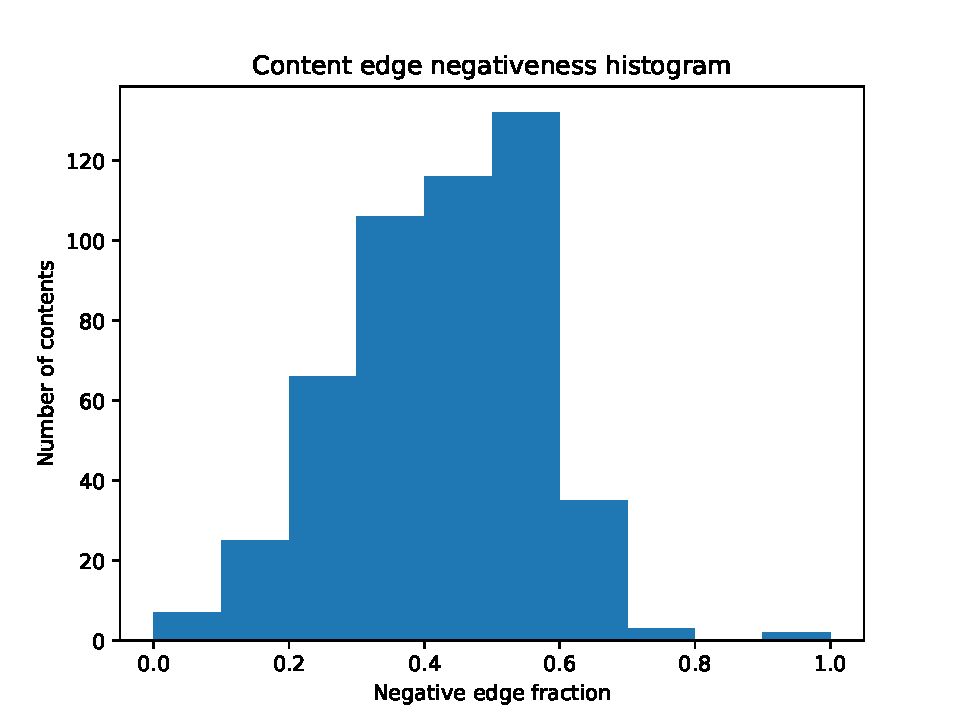
\includegraphics[width=\textwidth]{tex/out/nytimes700/neg-fraction-content-hist.pdf}
			\caption{$\eta(C)$ of @nytimes}
			\label{fig:nytimes-content-eta}
		\end{subfigure}
		\begin{subfigure}[b]{0.4\textwidth}
			\centering
			\includegraphics[width=\textwidth]{tex/out/nytimes700/neg-fraction-thread-hist.pdf}
			\caption{$\eta(T)$ for @nytimes}
			\label{fig:nytimes-thread-eta}
		\end{subfigure}
		\begin{subfigure}[b]{0.4\textwidth}
			\centering
			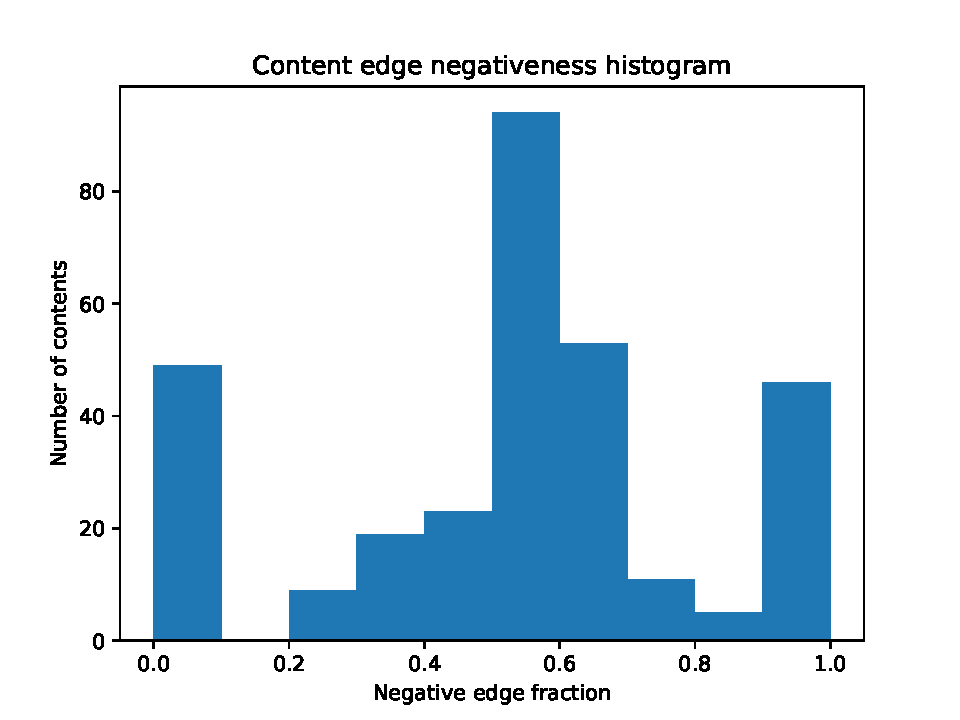
\includegraphics[width=\textwidth]{tex/out/foxnews2000/neg-fraction-content-hist.pdf}
			\caption{$\eta(C)$ of @foxnews}
			\label{fig:foxnews-content-eta}
		\end{subfigure}
		\begin{subfigure}[b]{0.4\textwidth}
			\centering
			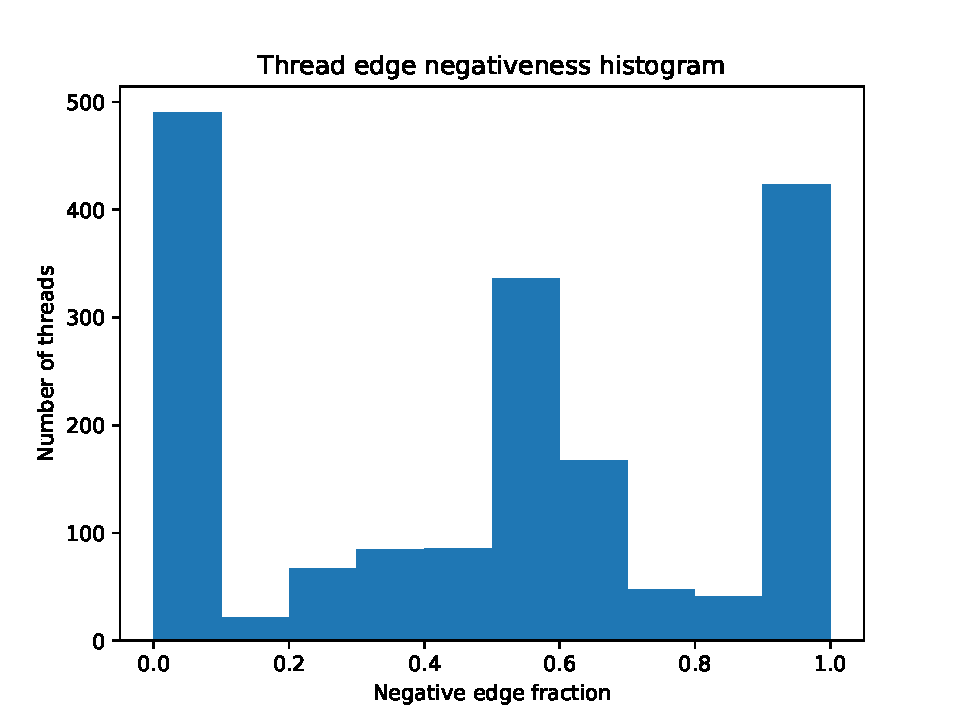
\includegraphics[width=\textwidth]{tex/out/foxnews2000/neg-fraction-thread-hist.pdf}
			\caption{$\eta(T)$ for @foxnews}
			\label{fig:foxnews-thread-eta}
		\end{subfigure}
		\begin{subfigure}[b]{0.4\textwidth}
			\centering
			% 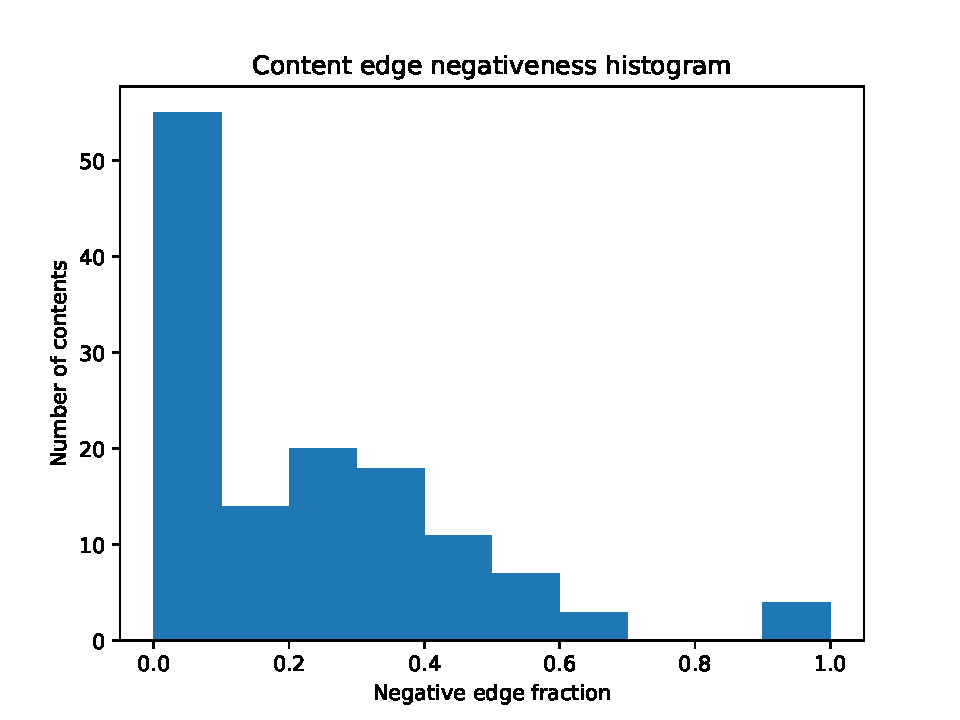
\includegraphics[width=\textwidth]{tex/out/CNN700/neg-fraction-content-hist.pdf}
			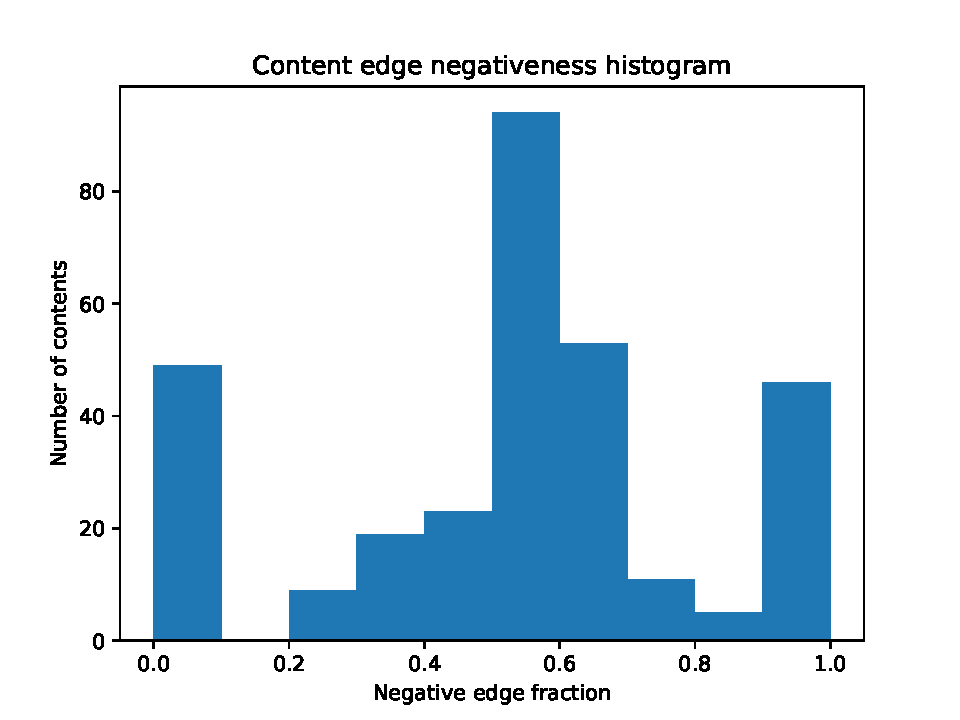
\includegraphics[width=\textwidth]{tex/out/foxnews2000/neg-fraction-content-hist.pdf}
			\caption{$\eta(C)$ of @CNN}
			\label{fig:CNN-content-eta}
		\end{subfigure}
		\begin{subfigure}[b]{0.4\textwidth}
			\centering
			% \includegraphics[width=\textwidth]{tex/out/CNN700/neg-fraction-thread-hist.pdf}
			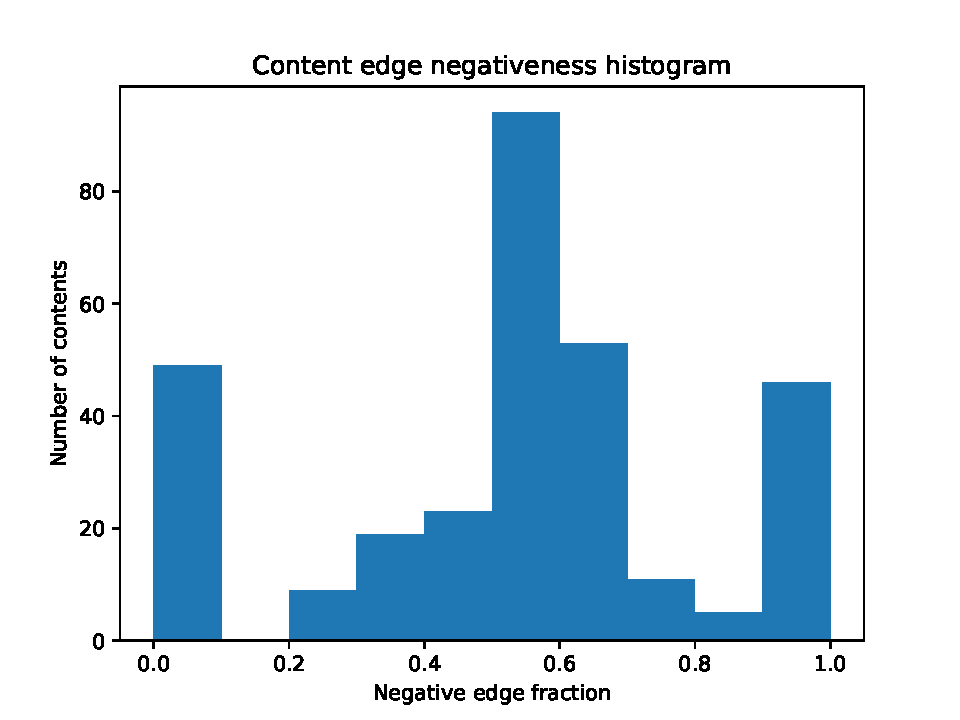
\includegraphics[width=\textwidth]{tex/out/foxnews2000/neg-fraction-content-hist.pdf}
			\caption{$\eta(T)$ for @CNN}
			\label{fig:CNN-thread-eta}
		\end{subfigure}
		\caption{$\eta(C)$ and $\eta(T)$ distribution for many datasets}
		\label{fig:eta-content-thread}
	\end{center}
\end{figure}

\bigskip
For verifying the reliability of the definition of \emph{controversial} content
we also looked at the fraction of negative edges for different datasets, each
associated to a different kind of content, which we report in
\autoref{tab:eta-subreddits}.

This results show an intuitive associations between the fraction of negative edges in the
graph and the topic discussed: politics contents
(r/politics and r/asktrumpsupporters) are generally the ones generating greater
controversy, and so do also related discussions (r/economics and r/climate) and
football. Subreddits in which discussion over technologies and sciences
predominate generally have less negative interactions between the users.

\begin{table}
	\centering
	\caption[Fraction of negative edges in different subreddits]{Fraction of negative edges for datasets build on different
		subreddits, each for $200$ contents}
	\label{tab:eta-subreddits}
	{\small
		\begin{tabular}{c | p{6cm} | c}
			r/cats               & Pictures and videos about cats                & \num{0.16922540125610608} \\
			\hline
			r/Covid19            & Scientific discussion of the pandemic         & \num{0.2981398553220806}  \\
			\hline
			r/programming        & Computer Programming discussions              & \num{0.30264993026499304} \\
			\hline
			r/climate            & News about climate and related politics       & \num{0.391787072243346}   \\
			\hline
			r/Football           & News, Rumours, Analysis about \mbox{football} & \num{0.41103067250904934} \\
			\hline
			r/Economics          & News and discussion about economics           & \num{0.41730200715730514} \\
			\hline
			r/Politics           & News and discussion about U.S. politics       & \num{0.5112245929821013}  \\
			\hline
			r/AskTrumpSupporters & {Q\&A between Trump supporters and non
			supporters}          & \num{0.5329949238578681}                                                  \\
		\end{tabular}
	}
\end{table}

\bigskip
Furthermore, we verified the association between a content $C$ and its
$\eta(C)$ by studying how its sum of weights of the edges relates to the number
of interactions happening for $C$ itself (see \autoref{fig:edge-sum-n-interactions}).

\begin{figure}
	\begin{center}
		\begin{subfigure}[b]{0.4\textwidth}
			\centering
			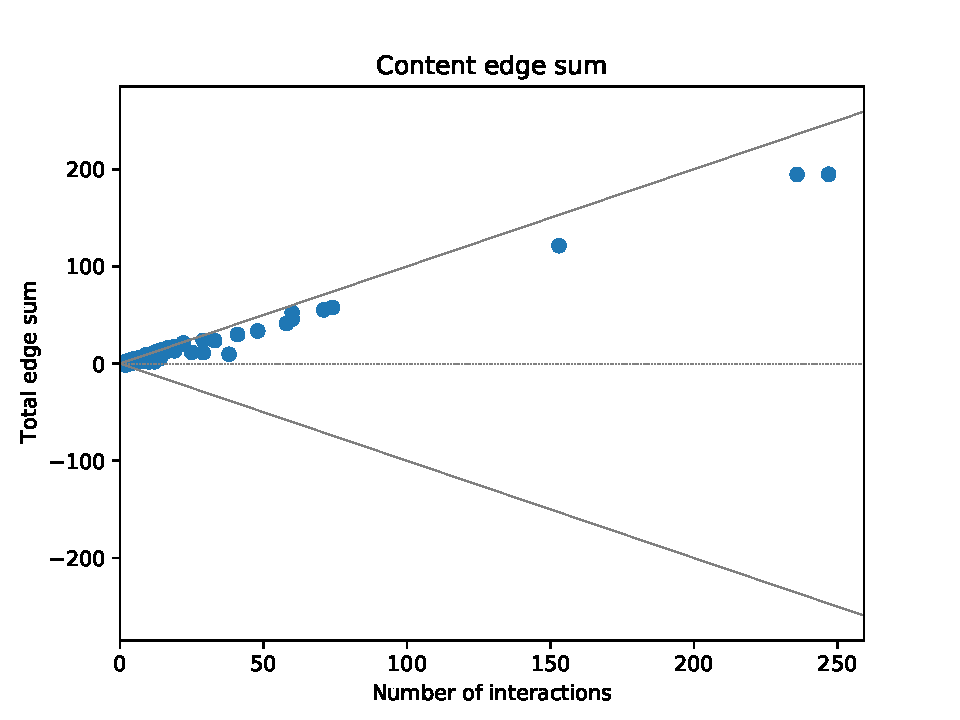
\includegraphics[width=\textwidth]{tex/out/cats200/edge-sum-n-interactions.pdf}
			\caption{r/cats}
			\label{fig:tex/out/cats200/edge-sum-n-interactions.pdf}
		\end{subfigure}
		\begin{subfigure}[b]{0.4\textwidth}
			\centering
			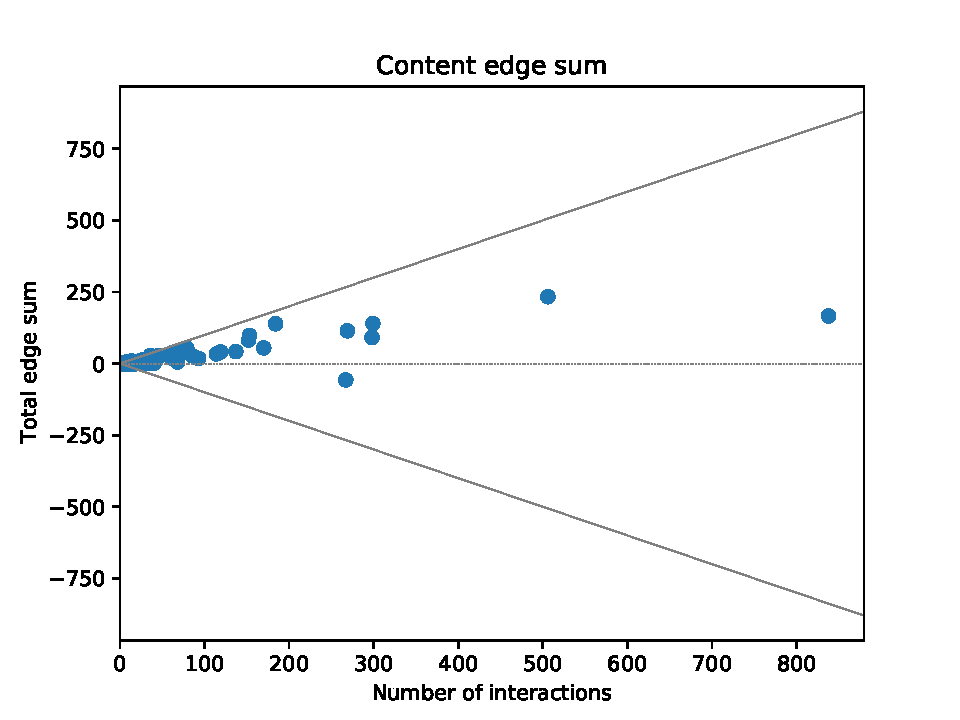
\includegraphics[width=\textwidth]{tex/out/covid19200/edge-sum-n-interactions.pdf}
			\caption{r/covid19}
			\label{fig:tex/out/covid19200/edge-sum-n-interactions.pdf}
		\end{subfigure}
		\begin{subfigure}[b]{0.4\textwidth}
			\centering
			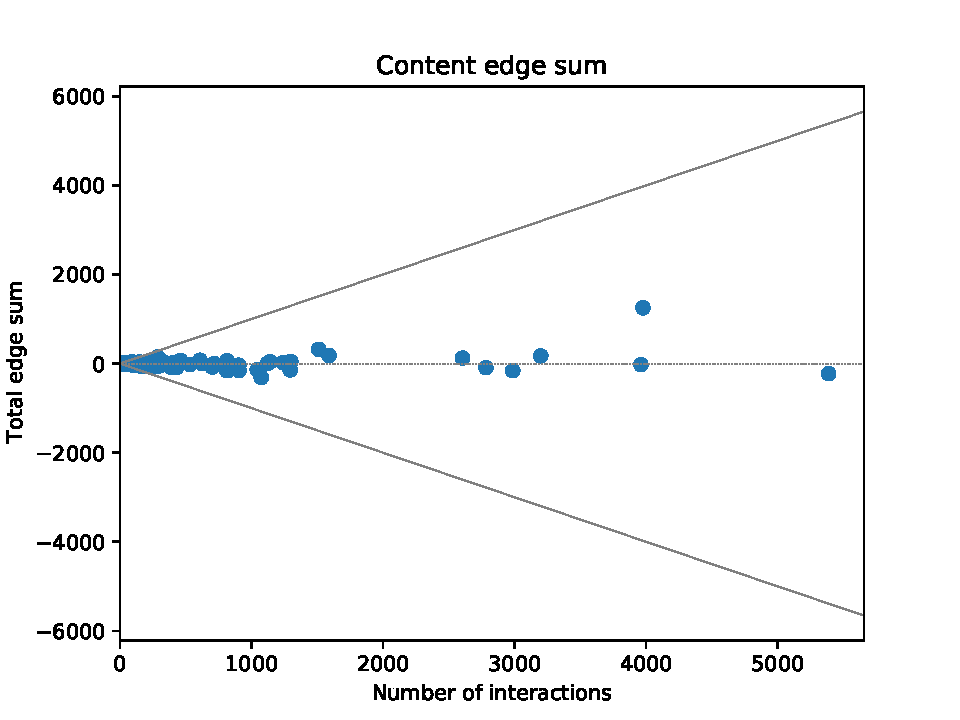
\includegraphics[width=\textwidth]{tex/out/politics200/edge-sum-n-interactions.pdf}
			\caption{r/politics}
			\label{fig:tex/out/cats200/edge-sum-n-interactions.pdf}
		\end{subfigure}
		\begin{subfigure}[b]{0.4\textwidth}
			\centering
			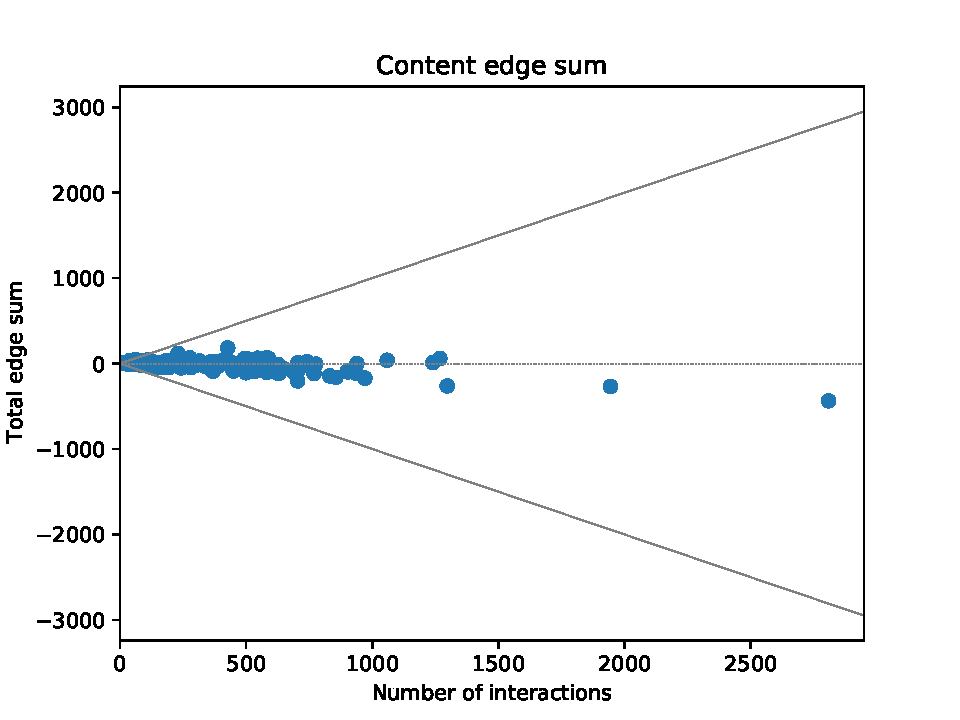
\includegraphics[width=\textwidth]{tex/out/asktrumpsupporters200/edge-sum-n-interactions.pdf}
			\caption{r/asktrumpsupporters}
			\label{fig:tex/out/covid19200/edge-sum-n-interactions.pdf}
		\end{subfigure}
	\end{center}
	\caption[Sum edges over number of interactions for many datasets]{Plots of
		sum of the edges weights over the number of interaction for contents
		from different datasets/subreddits}
	\label{fig:edge-sum-n-interactions}
\end{figure}

This plots confirm the previous observation and, more specifically, show that
the sum of the weights of the edges (which is easy to see it is closely related
to the $\eta(C)$ of $C$) for contents related to the same topic is distributed in a pattern which is very close to that of a line with rare or no outliers.
This is even more clearly visible when plotting the histogram of $\eta(C)$ for the contents in the dataset
(\autoref{fig:eta-distribution-content}), with most of the contents having a
$\eta(C)$ which is very similar to the fraction of negative edges in the graph.

\begin{figure}
	\begin{center}
		\begin{subfigure}[b]{0.4\textwidth}
			\centering
			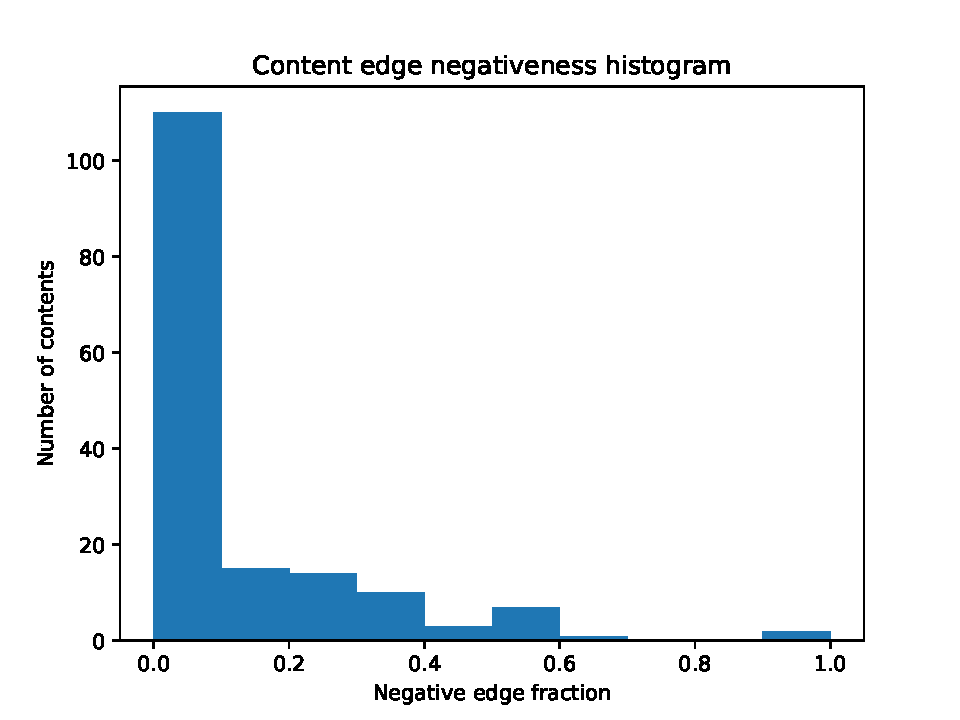
\includegraphics[width=\textwidth]{tex/out/cats200/neg-fraction-content-hist.pdf}
			\caption{r/cats}
			\label{fig:tex/out/cats200/neg-fraction-content-hist.pdf}
		\end{subfigure}
		\begin{subfigure}[b]{0.4\textwidth}
			\centering
			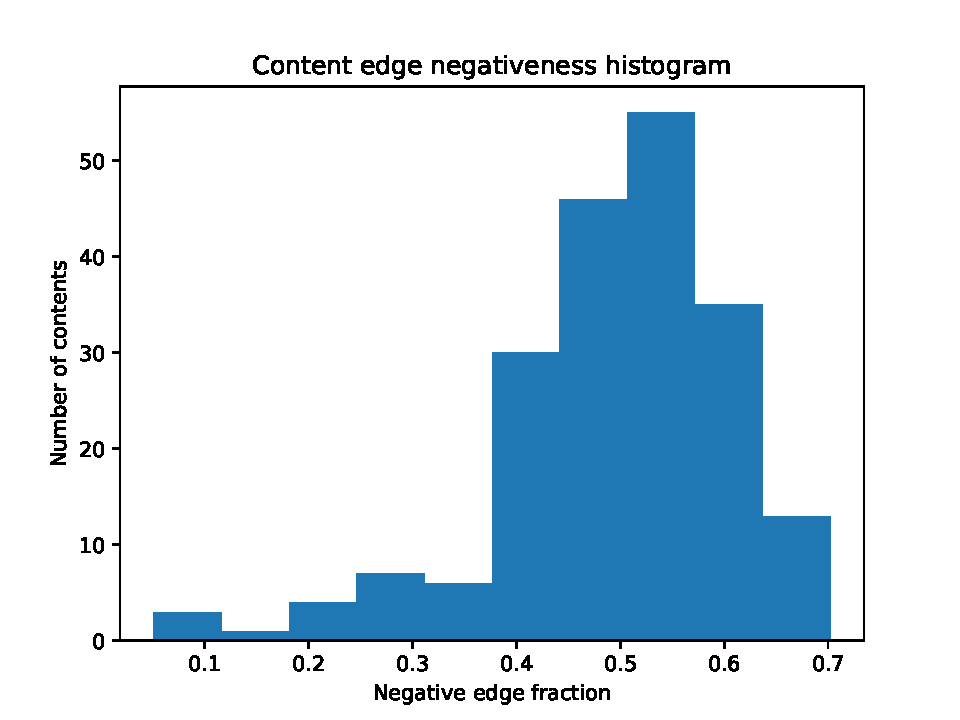
\includegraphics[width=\textwidth]{tex/out/asktrumpsupporters200/neg-fraction-content-hist.pdf}
			\caption{r/asktrumpsupporters}
			\label{fig:asktrump-hist-eta}
		\end{subfigure}
	\end{center}
	\caption{$\eta(C)$ distribution for $2$ of the datasets shown in
		\autoref{fig:edge-sum-n-interactions}}
	\label{fig:eta-distribution-content}
\end{figure}


\subsection{Algorithms implementation efficiency}%
\label{sub:algorithm_efficiency}

% todo:
% - time limitations of exact algorithms
% - describe beta algorithm and effect of beta, real world data
% - time efficiency of the greedy algorithms, real world data

\subsection{Tests on synthetic data}%
\label{sub:testing_on_synthetic_data}

For studying how the model behaves in controlled situations we define a
parametrized model based on the Information Spread model
(\autoref{ssub:information_spread_model}).

We choose $\beta _{a} = 1$, meaning that all nodes will be active in each
thread/layer. This a
simplifying assumption which allows us to have a better grasp of the results.
Because of this choice the values $\beta _n = 1$, $\theta = 1$ and
\begin{equation}
	\phi_{rs}  =
	\begin{cases}
		1 \; & \text{if } r = s  \\
		0 \; & \text{otherwise }
	\end{cases}
\end{equation}
do not influence the structure of the model.

We also choose $\omega ^{-} _{rs}$ and $\omega ^{+} _{rs} $ to be dependant on
the \emph{noise} variable $x$
\begin{equation}
	\omega_{rs}^{+}   =
	\begin{cases}
		1 - x \;        & \text{if } r = s  \\
		\frac{x}{4}  \; & \text{otherwise }
	\end{cases}
\end{equation}
\begin{equation}
	\omega_{rs}^{-}   =
	\begin{cases}
		x \;                & \text{if } r = s  \\
		\frac{1 - x}{4}  \; & \text{otherwise }
	\end{cases}
\end{equation}

In absence of noise ($x = 0$) we will generate threads whose communities are
positive cliques and all the edges between vertices in different communities
are negative.

We will compare different techniques for reconstructing the communities (which,
in this case, we will consider as corresponding to a community). The
general approach involves calling an algorithm (generally any of the methods
presented in \autoref{ch:solving}) returning a set of users $U
	\subseteq V$ which will be labeled according to the majority of its members
(by looking at the ground-truth assignment) and from the graph the edges
contributing to $\xi(U)$ are removed.
After repeating $n$ times this process, where
$n$ is the number of communities in the model, we compare the
compare the ground-truth and the predictions through the Jaccard coefficient and the Adjusted
RAND index\footnotemark.

\footnotetext{The Adjusted RAND index is a measure of similarity between
	different clusterings. It is based on the RAND index, which compares
	the number of agreeing pairs in the $2$ solutions; the Adjusted one corrects
	the Rand Index "by chance", i.e. compares it to the expected index
	(from a random assignment). For more details please
	refer to \cite{CharuC.Aggarwal2013}}

What we expect is that, as the value of $x$ increases, the produced threads
will have generally more negative edges inside a community and more positive
edges between different communities, making it more difficult for our
algorithms to spot a set of vertices corresponding to a community.

We compared the scores obtained with the \acrshort{MIP} for the \acrshort{ECP}
(\autoref{sub:a_mip_model_for_the_ecp}), the Rounding algorithm
(\autoref{ssub:rounding_algorithm}) and the $2$ alternative problems on the
\acrshort{TPA} Graph (\autoref{ssub:the_tpa_graph}). Due to the presence of the
\acrshort{MIP} model this group of experiments have been carried out on very
small graphs. % todo specify how small

We then focused on the performances of the Rounding Algorithm on bigger
datasets.

% - describe rounding algorithm: when does it fail?
% - observation on the results (how does it depend on the number of threads and
%   on the number of nodes in each community?

\subsection{Detecting real-world echo chambers}%
\label{sub:detecting_real_echo_chambers}

% report some real world echo chambers

\subsection{The r/asktrumpsupporters case}%
\label{sub:the_r_asktrumpsupporters_case}


\section{Validity and reliability analysis}
\label{sec:reliability_analysis}

% todo: talk about the limitations of the thread-content model in the reddit
% environment (see slides of 02.08)
